\documentclass[12pt]{article}

\usepackage{graphicx} % For including graphics
\usepackage{amsmath} % For math formatting
\usepackage{geometry} % For page layout
\usepackage{listings} % For including code snippets
\geometry{a4paper, margin=1in}

\title{Effect of Lead Thickness on Radiation Detection}
\author{Enrique Rivera Jr. \\
        Physics Undergraduate, \\ 
        The University of Texas at Austin}
\date{\today}

\begin{document}

\maketitle

\begin{abstract}
    In our investigation, we examined how varying thicknesses of lead 
    influence the detection of radiation emitted by Cobalt-60, a widely utilized radioactive isotope. 
    Utilizing a scintillator, we quantified the radiation intensity across different lead shields. 
    Our observations revealed a predictable decline in radiation intensity with increased lead thickness, 
    aligning with theoretical expectations. Notably, this attenuation follows an exponential trend, 
    underscoring the complex dynamics of radiation shielding. These insights contribute valuable knowledge towards 
    optimizing radiation protection materials, emphasizing the exponential nature of radiation attenuation 
    through lead. This understanding is crucial for designing more effective shielding strategies in 
    both medical and industrial applications, enhancing safety protocols against radioactive exposure.
\end{abstract}

\section{Introduction}
    The study of radioactive decay remains a cornerstone in understanding nuclear processes, 
    with Cobalt-60 frequently serving as a pivotal subject due to its prevalent use in both 
    medical and industrial applications. This isotope's emission characteristics offer a 
    valuable window into the dynamics of gamma radiation, a form of energy crucial in a 
    variety of fields. The attenuation of this radiation by shielding materials, particularly lead, 
    is of paramount importance for ensuring safety and efficacy in these applications. 
    Lead is traditionally favored for its high density and atomic number, which contribute to 
    its effectiveness in absorbing gamma radiation. However, the relationship between lead thickness 
    and radiation attenuation is not merely a matter of linear correlation but involves more 
    complex interactions that significantly influence shielding design. This experiment aims to elucidate 
    these interactions by systematically varying the thickness of lead shielding to observe its impact 
    on radiation detection from Cobalt-60, thereby providing insights that could refine our 
    approach to radiation protection.

    \section{Experimental Setup and Procedure}
        \subsection{Materials and Equipment}
            The primary materials and equipment used in this experiment include:
            \begin{itemize}
                \item Cobalt-60 radioactive source
                \item Lead sheets of varying thicknesses in mm (1.530, 3.060, 5.860, 8.670, 14.500, 20.300, 29.000) 
                \item Scintillator
                \item Multi-channel analyzer (MCA) and single-channel analyzer (SCA)
                \item Data acquisition Software (Maestro)
                \item Python programming environment (miniconda with Python notebooks)
            \end{itemize}
            
        \subsection{Apparatus}
            The experimental setup consists of a Cobalt-60 source, a Radiation Detection Module, and lead sheets of varying thicknesses. 
            The Cobalt-60 source emits gamma radiation, which is detected by the scintillator. 
            The lead sheets are placed between the source and the scintillator to measure the attenuation of the radiation. 
            The Radiation Detection Module is connected to a data acquisition system(Maestro), which records the intensity of the radiation over time in a histogram plot. 
            The data is then passed to a Python program, which allows us to measure the radiation intensity at different lead thicknesses with our plot analysis.
            
            \begin{figure}[!htb]
                \centering
                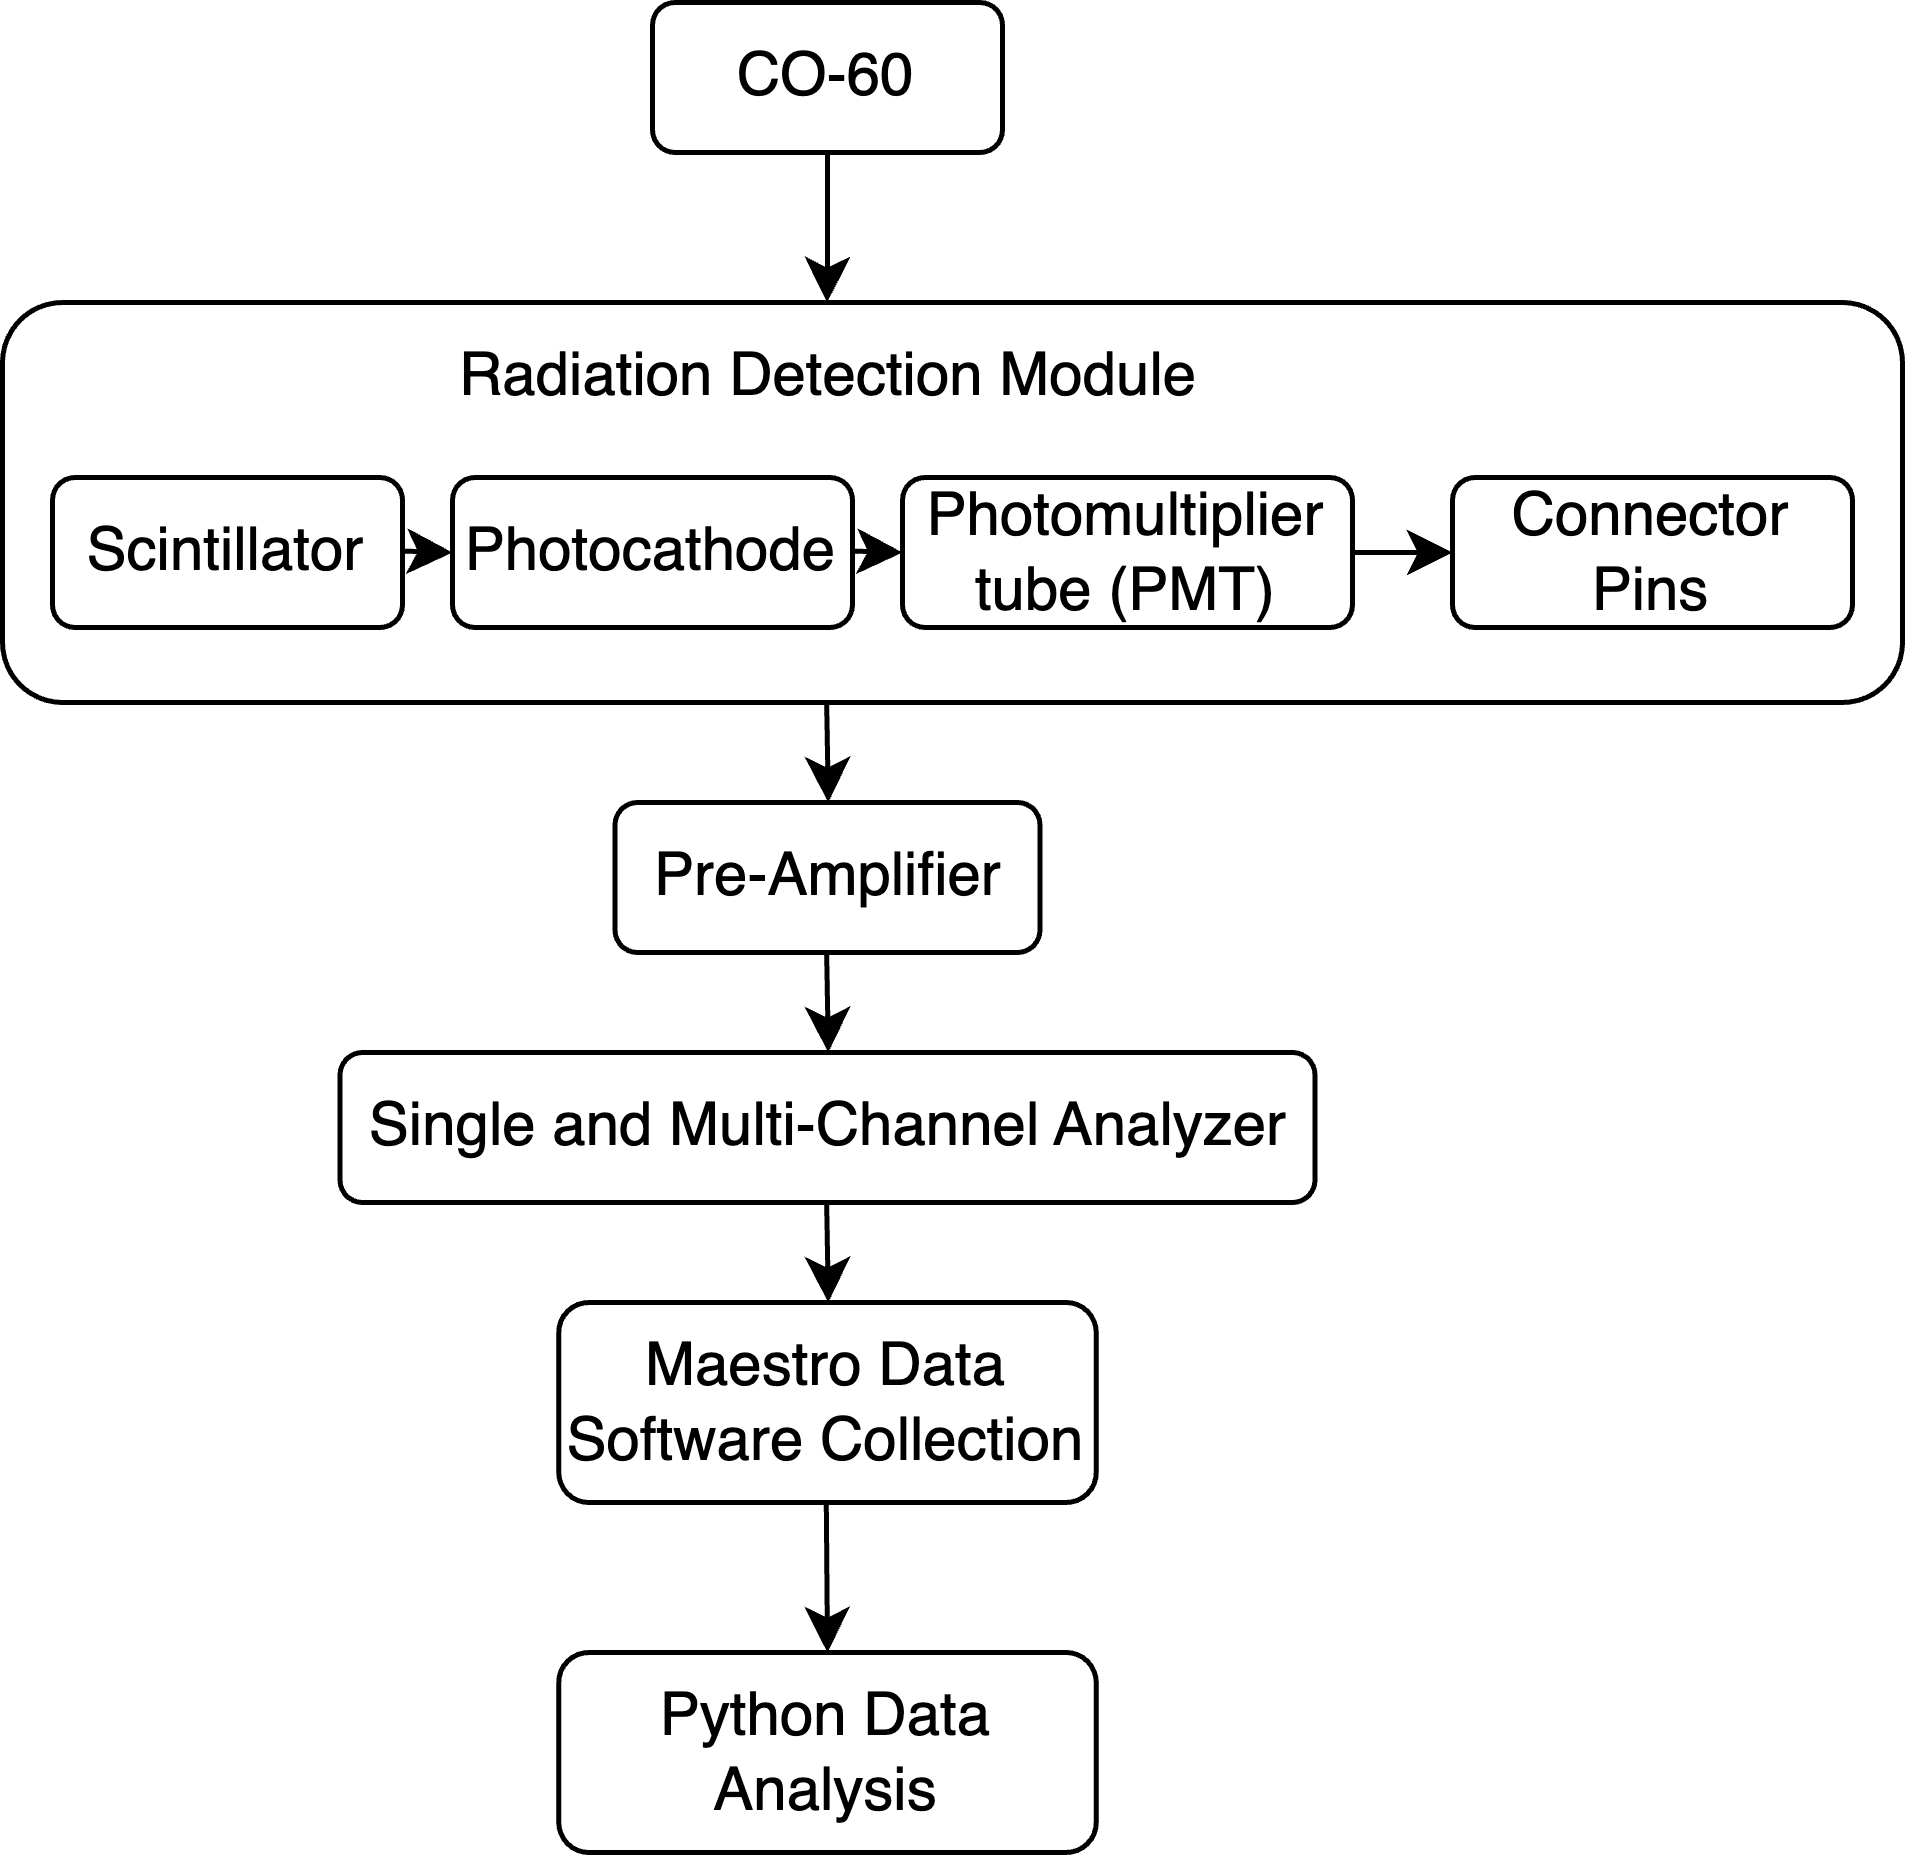
\includegraphics[width=0.5\textwidth]{./img/other/Lab1 Apparatus.png}
                \caption{Apparatus Flow Chart}
                \label{fig:graph1}
            \end{figure}

        \subsection{Scintillator}
            The scintillator is a device that detects radiation by converting the energy of incoming photons into visible light. 
            This light is then detected by a photomultiplier tube, which amplifies the signal and converts it into an electrical pulse. 
            The scintillator used in this experiment is a sodium iodide (NaI) crystal, which is commonly used for detecting gamma radiation. 
            The crystal is coupled to a photomultiplier tube, which amplifies the light signal and converts it into an electrical pulse. 

        \subsection{Photomultiplier to Electronic Multiplier}
            The photomultiplier tube is a device that converts the light signal from the scintillator into an electrical pulse. 
            It consists of a series of dynodes, which are metal electrodes that are held at successively higher voltages. 
            When a photon strikes the first dynode, it releases an electron, which is then accelerated towards the next dynode. 
            This process is repeated at each dynode, resulting in a cascade of electrons that is amplified at each stage. 
            The final output is a large number of electrons, which is then converted into an electrical pulse. 
            This pulse is then passed to a electronic preamplifier to be then processed by the data acquisition system, 
            which records the number of pulses over a given time interval. 
            This allows us to measure the intensity of the radiation emitted by the Cobalt-60 source.

            \begin{figure}[!htb]
                \centering
                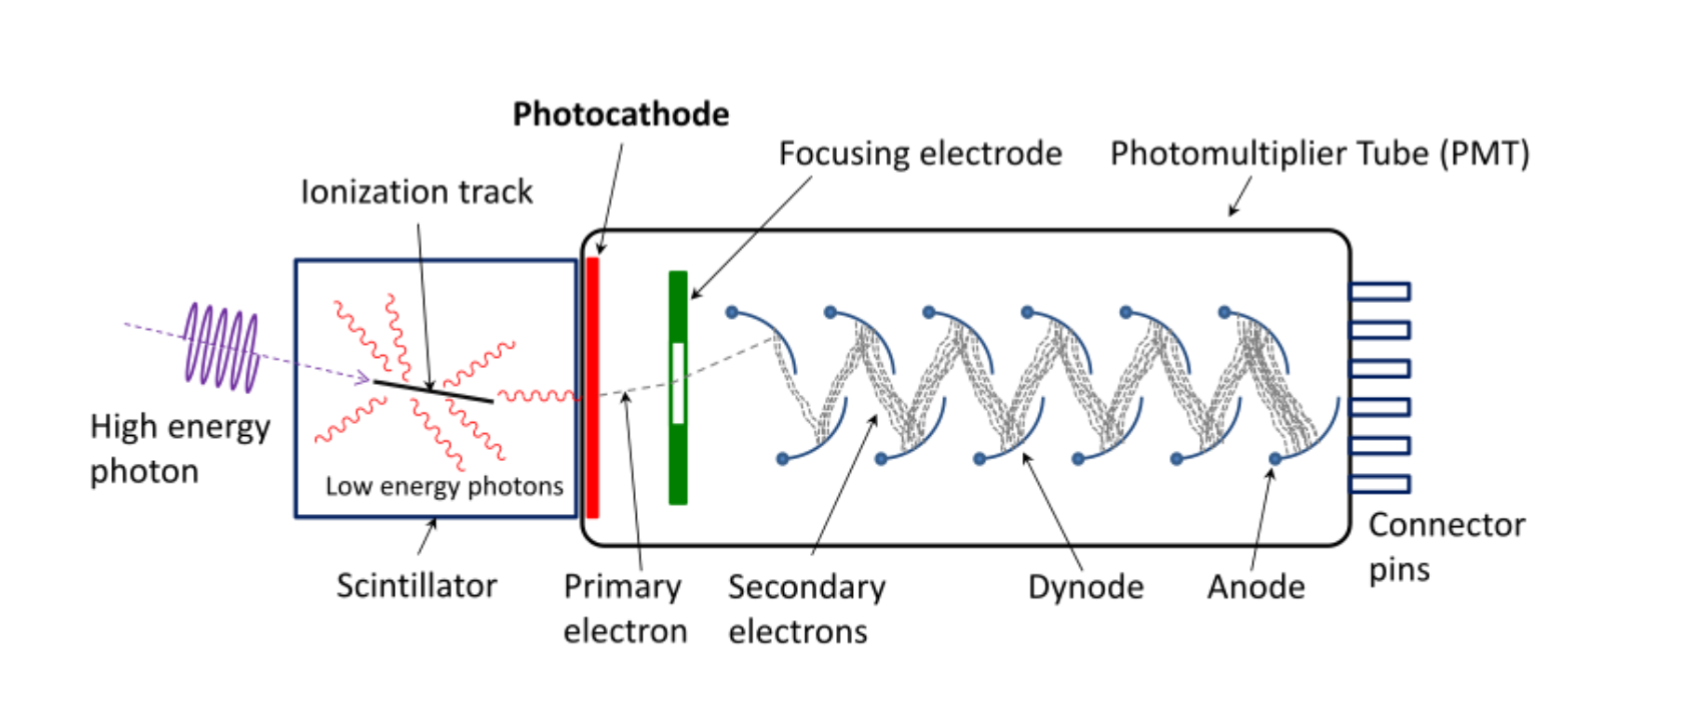
\includegraphics[width=0.9\textwidth]{./img/other/module.png}
                \caption{Radiation Detection Module [1]}
                \label{fig:Radiation Detection Module [1]}
            \end{figure}
            
        \subsection{Single and Multi-Channel Analyzer (Cobalt-60 Gamma Ray Spectrum)}
            The single-channel analyzer (SCA) is a device that allows us to select a specific range of energy from the photomultiplier tube. 
            This is useful for filtering out background radiation and other unwanted signals. 
            The multi-channel analyzer (MCA) is a device that allows us to record the number of pulses at each energy bin. 
            This allows us to measure the intensity of the radiation emitted by the Cobalt-60 source as a histogram 
            where number of occurrences for a specific energy bin is measure as a count. 
            The MCA and the SCA is connected to a computer, which allows us to record and visualize the data. The MCA creates a spectrum of the detected events
            The data is then processed using a Python program, which allows us to compare the radiation intensity at different lead thicknesses.
            
        \subsection{Data Collection}
            The data acquisition system record the intensity of the radiation emitted by the Cobalt-60 source at different lead thicknesses. 
            The data is then processed using a Python program, where the the data first was exported from the data acquisition system.
            Initially, the data was exported as a .lvm file from the data acquisition system and then converted to a .csv file. 
            Subsequently, it was read into a Python program using the Pandas library.
            From data, graphs are generate to show the radiation intensity at different lead thicknesses. 
            These graphs are then analyzed to determine the relationship between lead thickness and radiation attenuation using 
            Possion distribution fit on the histograms of the data.
            
            \lstset{language=Python}
            \lstset{frame=lines}
            \lstset{caption={LVM to CSV Code Snippet}}
            \lstset{label={lst:code_direct}}
            \lstset{basicstyle=\footnotesize}
            \begin{lstlisting}

                def lvm_to_csv(lvm_filename, csv_filename):
                # Remove the head data from the LVM file first
                # Open the LVM file for reading
                with open(lvm_filename, 'r') as lvm_file:
                    # Read the entire file into memory
                    lines = lvm_file.readlines()
            
                data_lines = lines
            
                # Open the CSV file for writing
                with open(csv_filename, 'w', newline='') as csv_file:
                    writer = csv.writer(csv_file)
                    
                    colums = "Time	Col1	Col2	Scale"
                    writer.writerow( colums.strip().split() )
                    
                    
                    # Write data to CSV file
                    for line in data_lines:
                        # Split the line into values based on whitespace
                        values = line.strip().split()
                        writer.writerow(values)
            \end{lstlisting}
                

\section{Results}
    Present the data obtained from the experiment. Include your Python-generated graphs here. Use the following syntax to include images:
    

\section{Conclusion}
    Summarize the main findings of the experiment, the implications of these findings, and potential areas for further research.

\section{References}
    List the references cited in your report.

\end{document}
